\chapter{Benchmarking}

A set of 51 huge problems was chosen from the \ac{tptp} archive to be used for the benchmarks. Each problem contains 3,341,984 formulae. The choice of those problems was because they have a huge shared knowledge base and each problem is just a different conjecture. Table~\ref{Table:BenchmarkingProblems} shows the list of the problem names chosen for the benchmarks.
\begin{table}[ht]
  \begin{center}
    \begin{tabular}{c|c||c|c}
      \toprule
      Problem Name & Number Of Formulae & Problem Name & Number Of Formulae \\
      \midrule
      CSR025+6.p   & 3,341,984          & CSR050+6.p   & 3,341,984 \\
      CSR026+6.p   & 3,341,984          & CSR051+6.p   & 3,341,984 \\
      CSR027+6.p   & 3,341,984          & CSR052+6.p   & 3,341,984 \\
      CSR028+6.p   & 3,341,984          & CSR053+6.p   & 3,341,984 \\
      CSR029+6.p   & 3,341,984          & CSR054+6.p   & 3,341,984 \\
      CSR030+6.p   & 3,341,984          & CSR055+6.p   & 3,341,984 \\
      CSR031+6.p   & 3,341,984          & CSR056+6.p   & 3,341,984 \\
      CSR032+6.p   & 3,341,984          & CSR057+6.p   & 3,341,984 \\
      CSR033+6.p   & 3,341,984          & CSR058+6.p   & 3,341,984 \\
      CSR034+6.p   & 3,341,984          & CSR059+6.p   & 3,341,984 \\
      CSR035+6.p   & 3,341,984          & CSR060+6.p   & 3,341,984 \\
      CSR036+6.p   & 3,341,984          & CSR061+6.p   & 3,341,984 \\
      CSR037+6.p   & 3,341,984          & CSR062+6.p   & 3,341,984 \\
      CSR038+6.p   & 3,341,984          & CSR063+6.p   & 3,341,984 \\
      CSR039+6.p   & 3,341,984          & CSR064+6.p   & 3,341,984 \\
      CSR040+6.p   & 3,341,984          & CSR065+6.p   & 3,341,984 \\
      CSR041+6.p   & 3,341,984          & CSR066+6.p   & 3,341,984 \\
      CSR042+6.p   & 3,341,984          & CSR067+6.p   & 3,341,984 \\
      CSR043+6.p   & 3,341,984          & CSR068+6.p   & 3,341,984 \\
      CSR044+6.p   & 3,341,984          & CSR069+6.p   & 3,341,984 \\
      CSR045+6.p   & 3,341,984          & CSR070+6.p   & 3,341,984 \\
      CSR046+6.p   & 3,341,984          & CSR071+6.p   & 3,341,984 \\
      CSR047+6.p   & 3,341,984          & CSR072+6.p   & 3,341,984 \\
      CSR048+6.p   & 3,341,984          & CSR073+6.p   & 3,341,984 \\
      CSR049+6.p   & 3,341,984          & CSR111+6.p   & 3,341,984 \\
      CSR074+6.p   & 3,341,984          &              &           \\
      \bottomrule
    \end{tabular}
  \end{center}
\caption{Benchmarking Problems}
\label{Table:BenchmarkingProblems}
\end{table}

The benchmarks were between the plain normal eprover and the server running in a single strategy mode. The axioms are passed to the axiom filter before passing it to the plain E prover. The server used the same strategy that was used in the axiom filter for a fair comparison with the plain prover. The two of them used a memory limit of 1024MB and a 30 seconds time limit for the proof search. The benchmarks ran over the first 5, 10, 20, 30, 40 and 51 problems. The time taken for the two modes to solve all the problems in each benchmark is noted. Also the number of problems solved by the two mode is noted.

\begin{figure}[ht!]
  \centering
  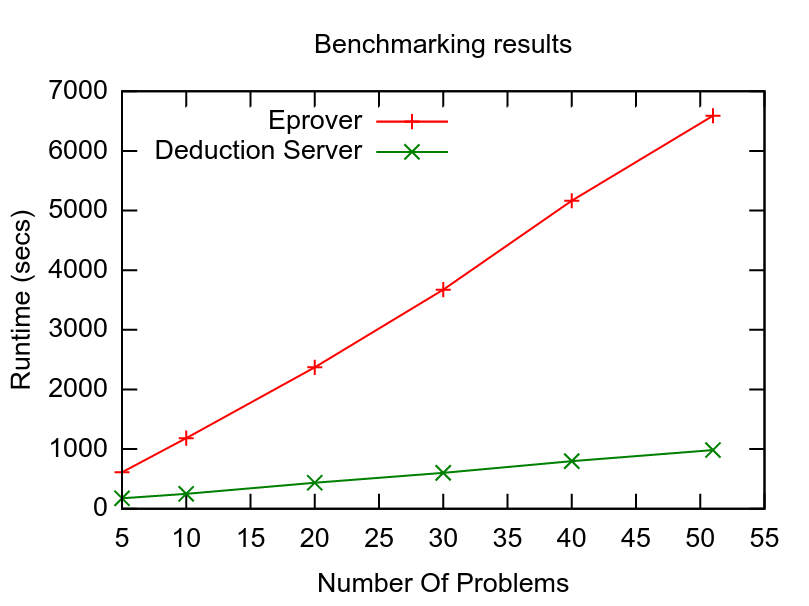
\includegraphics[width=150mm]{graphics/BenchmarkingResults.png}
  \caption{Benchmarking Results\label{benchmarking_results}}
\end{figure}

The results in Figure~\ref{benchmarking_results} shows a huge difference between the single strategy server mode and the normal eprover. That is because parsing the huge knowledge base takes large amount of time which is done in the normal eprover once for each problem. In the single strategy server mode the huge axiom set is parsed only once and kept in the server's memory and multiple queries ran against this axiom set. Therefor the per-processing time of each problem in the single strategy server mode is amortized over multiple runs.

Both modes solved the same 41 problems out of the 51 problems used in the benchmarks. This means that the server mode has a performance advantage over the plain E prover without affecting its efficiency.
